\documentclass[12pt]{article}
\usepackage[T1, T2A]{fontenc}
\usepackage[utf8]{inputenc}
\usepackage[russian]{babel}
\usepackage{hyperref}
\usepackage{graphicx}
\graphicspath{ {../Images/} }

\author{Григорий Матюхин}
\date{\today}
\title{Лабораторная работа \textnumero3.\\Настройка прав доступа}

\begin{document}
\maketitle
\newpage
\tableofcontents
\newpage
\section{Цель работы}
Получение навыков настройки базовых и специальных прав доступа для групп пользователей в операционной системе типа Linux.

\section{Последовательность выполнения работы}

\subsection{Управление базовыми разрешениями}
Требуется создать структуру каталогов с разными разрешениями доступа для
разных групп пользователей.
\begin{enumerate}
	\item Откройте терминал с учётной записью \texttt{root}:
	\item В корневом каталоге создайте каталоги \texttt{/data/main} и \texttt{/data/third}:
	\item Прежде чем устанавливать разрешения, измените владельцев этих каталогов с \texttt{root} на \texttt{main} и \texttt{third} соответственно:
	      \\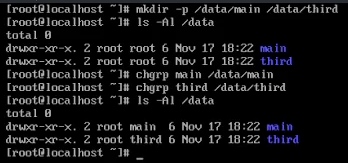
\includegraphics{1.png}
	\item Установите разрешения, позволяющие владельцам каталогов записывать файлы в эти каталоги и запрещающие доступ к содержимому каталогов всем другим пользователям и группам:
	      \\
\includegraphics{2.png}
	\item В другом терминале перейдите под учётную запись пользователя bob:
	\item Под пользователем \texttt{bob} попробуйте перейти в каталог \texttt{/data/main} и создать файл \texttt{emptyfile} в этом каталоге:
	\item Под пользователем \texttt{bob} попробуйте перейти в каталог \texttt{/data/third} и создать файл \texttt{emptyfile} в этом каталоге:
	      \\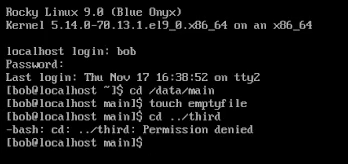
\includegraphics{3.png}
\end{enumerate}

\subsection{Управление специальными разрешениями}
Требуется, используя специальные разрешения для групп пользователей, обеспечить обмен файлами в общем для групп каталоге. При этом каталогу назначается бит идентификатора группы, а также \textit{sticky bit}.\\
\textbf{Sticky bit} — дополнительный атрибут файлов или каталогов в ОС типа Linux, применяющийся в основном для каталогов с целью защиты содержимого каталогов от повреждения или удаления пользователями, не являющимися их владельцами. Для установки этого атрибута используется утилита \texttt{chmod}. Восьмеричное значение \texttt{sticky bit}: \texttt{1000}, а символьное: \texttt{+t}.
\begin{enumerate}
	\item Откройте новый терминал под пользователем \texttt{alice}:
	\item Перейдите в каталог \texttt{/data/main}. Создайте два файла, владельцем которых является alice:
	      \\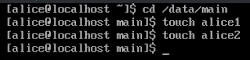
\includegraphics{4.png}
	\item В другом терминале перейдите под учётную запись пользователя \texttt{bob} (пользователь \texttt{bob} является членом группы \texttt{main}, как и \texttt{alice}):
	\item Перейдите в каталог \texttt{/data/main} и в этом каталоге введите \texttt{ls -l}. Вы увидите два файла, созданные пользователем \texttt{alice}. Попробуйте удалить файлы, принадлежащие пользователю \texttt{alice}. Убедитесь, что файлы будут удалены пользователем \texttt{bob}:
	      \\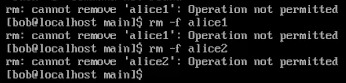
\includegraphics{5.png}
	\item В другом терминале перейдите под учётную запись пользователя \texttt{bob} (пользователь \texttt{bob} является членом группы \texttt{main}, как и \texttt{alice}):
	\item Создайте два файла, которые принадлежат пользователю \texttt{bob}:
	\item В терминале под пользователем root установите для каталога \texttt{/data/main} бит идентификатора группы, а также \textit{sticky bit} для разделяемого (общего) каталога группы:
	      \\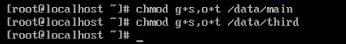
\includegraphics{6.png}
	\item В терминале под пользователем \texttt{alice} создайте в каталоге \texttt{/data/main} файлы \texttt{alice3} и \texttt{alice4}. Теперь вы должны увидеть, что два созданных вами файла принадлежат группе \texttt{main}, которая является группой-владельцем каталога \texttt{/data/main}.
	      \\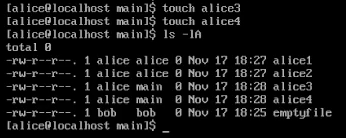
\includegraphics{7.png}
	\item В терминале под пользователем alice попробуйте удалить файлы, принадлежащие пользователю bob:
	      \\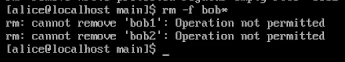
\includegraphics{8.png}
\end{enumerate}
Убедитесь, что \textit{sticky bit} предотвратит удаление этих файлов пользователем \texttt{alice}, поскольку этот пользователь не является владельцем этих файлов. Обратите внимание: поскольку пользователь \texttt{alice} является владельцем каталога \texttt{/data/main}, то он может удалить все свои файлы в любом случае.

\subsection{Управление расширенными разрешениями с использованием списков ACL}
Требуется установить для группы \texttt{third} разрешения на чтение в каталоге \texttt{/data/main}, а для группы \texttt{main} — разрешения на чтение в каталоге \texttt{/data/third}. Затем требуется установить права доступа по умолчанию, чтобы убедиться в правильности установки разрешений для новых элементов этих каталогов. Для этого будет использоваться пакет \texttt{acl} и команды \texttt{setfacl} (для установки прав) и \texttt{getfacl} (для просмотра установленных прав).
\begin{enumerate}
	\item Откройте терминал с учётной записью \texttt{root}:
	\item Установите права на чтение и выполнение в каталоге \texttt{/data/main} для группы \texttt{third} и права на чтение и выполнение для группы main в каталоге \texttt{/data/third}:
	\item Используйте команду \texttt{getfacl}, чтобы убедиться в правильности установки разрешений:
	      \\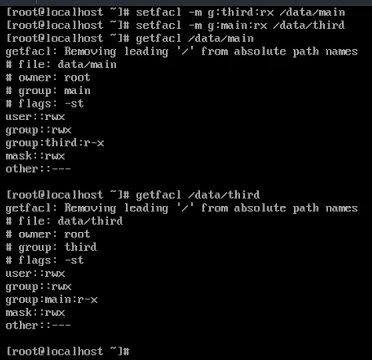
\includegraphics{9.png}
	\item Создайте новый файл с именем \texttt{newfile1} в каталоге \texttt{/data/main}. Используйте \texttt{getfacl /data/main/newfile1} для проверки текущих назначений полномочий. Какие права доступа у этого файла? Объясните, почему.\\
	      \\
\includegraphics{10.png}
	\item Установите \texttt{ACL} по умолчанию для каталога \texttt{/data/main}:
	\item Добавьте \texttt{ACL} по умолчанию для каталога \texttt{/data/third}:
	      \\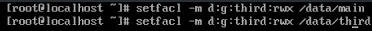
\includegraphics{11.png}
	\item Убедитесь, что настройки \texttt{ACL} работают, добавив новый файл в каталог \texttt{/data/main}. Используйте \texttt{getfacl /data/main/newfile2} для проверки текущих назначений полномочий.\\
	      \\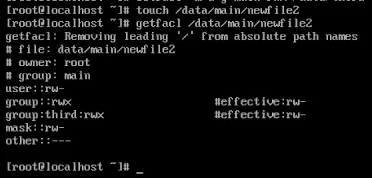
\includegraphics{12.png}
	\item Для проверки полномочий группы \texttt{third} в каталоге \texttt{/data/third} войдите в другом терминале под учётной записью члена группы \texttt{third}. Проверьте операции с файлами \texttt{/data/main/newfile1} и \texttt{/data/main/newfile2}. Проверьте, возможно ли осуществить запись в файлы.\\
	      \\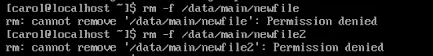
\includegraphics{13.png}
	      \\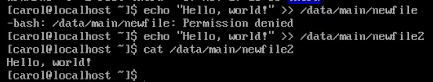
\includegraphics{14.png}
\end{enumerate}

\section{Контрольные вопросы}
\begin{enumerate}
	\item Как следует использовать команду \texttt{chown}, чтобы установить владельца группы для файла? Приведите пример.\\
	      \texttt{chown root /u} -- Поменять владельца \texttt{/u} на \texttt{root}.\\
	      \texttt{chown root:staff /u} -- То же самое, но также поменять группу на \texttt{staff}.\\
	      \texttt{chown :staff /u} -- Можно указать только группу.

	\item С помощью какой команды можно найти все файлы, принадлежащие конкретному пользователю? Приведите пример.\\
	      \texttt{find <directory> -user <user-name>}\\
	      \texttt{find ~/Documents -user bob}

	\item Как применить разрешения на чтение, запись и выполнение для всех файлов в каталоге \texttt{/data} для пользователей и владельцев групп, не устанавливая никаких прав для других? Приведите пример.\\
	      \texttt{chmod -R 770 ~/NoOutsiders} -- Рекурсивно поменяет разрешения для директории \texttt{NoOutsiders}.

	\item Какая команда позволяет добавить разрешение на выполнение для файла, который необходимо сделать исполняемым?\\
	      \texttt{chmod u+x <file-name>}

	\item Какая команда позволяет убедиться, что групповые разрешения для всех новых файлов, создаваемых в каталоге, будут присвоены владельцу группы этого каталога? Приведите пример.\\
	      \texttt{chmod g+s <directory>}\\
	      \texttt{chmod g+s /groups/group1}

	\item Необходимо, чтобы пользователи могли удалять только те файлы, владельцами которых они являются, или которые находятся в каталоге, владельцами которого они являются. С помощью какой команды можно это сделать? Приведите пример.\\
	      \texttt{chmod o+t <directory>}

	\item Какая команда добавляет \texttt{ACL}, который предоставляет членам группы права доступа на чтение для всех существующих файлов в текущем каталоге?
	      \texttt{setfacl -m g:groupname:rx <directory>}\\
	      \texttt{setfacl -m g:groupname:r <directory>/*}

	\item Что нужно сделать для гарантии того, что члены группы получат разрешения на чтение для всех файлов в текущем каталоге и во всех его подкаталогах, а также для всех файлов, которые будут созданы в этом каталоге в будущем? Приведите пример.\\
	      \texttt{setfacl -dm g:groupname:rx <directory>}

	\item Какое значение \texttt{umask} нужно установить, чтобы «другие» пользователи не получали какие-либо разрешения на новые файлы? Приведите пример.\\
	      \texttt{umask 007}

	\item Какая команда гарантирует, что никто не сможет удалить файл \texttt{myfile} случайно?
	      \texttt{chattr +i myfile}

\end{enumerate}

\section{Вывод}
В ходе выполнения данной работы я получил навыки настройки базовых и специальных прав доступа для групп пользователей в операционной системе типа Linux.

\end{document}
